\documentclass{article}
\usepackage{tikz}
\usetikzlibrary{positioning}

\begin{document}

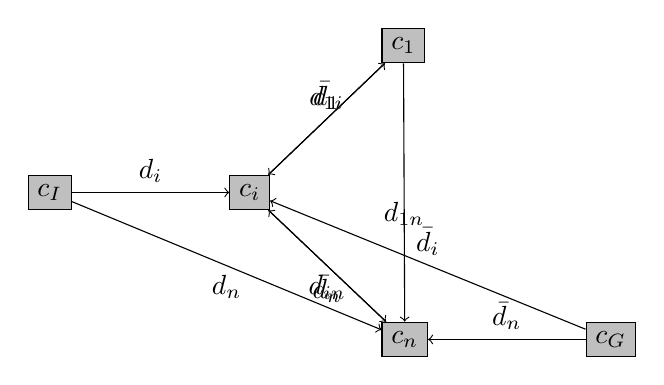
\begin{tikzpicture}[node distance=2cm]
    \node[draw, fill=gray!50] (cI) {$c_I$};
    \node[draw, fill=gray!50, right=of cI] (ci) {$c_i$};
    \node[draw, fill=gray!50, above right=of ci] (c1) {$c_1$};
    \node[draw, fill=gray!50, below right=of ci] (cn) {$c_n$};
    \node[draw, fill=gray!50, right=of cn] (cG) {$c_G$};

    \draw[->] (cI) -- node[above] {$d_i$} (ci);
    \draw[->] (ci) -- node[above] {$d_{1i}$} (c1);
    \draw[->] (c1) -- node[above] {$\bar{d}_1$} (ci);
    \draw[->] (ci) -- node[below] {$d_{in}$} (cn);
    \draw[->] (cn) -- node[below] {$\bar{d}_n$} (ci);
    \draw[->] (cI) -- node[below] {$d_n$} (cn);
    \draw[->] (cG) -- node[above] {$\bar{d}_i$} (ci);
    \draw[->] (cG) -- node[above] {$\bar{d}_n$} (cn);
    \draw[->] (c1) -- node[below] {$d_{1n}$} (cn);
\end{tikzpicture}

\end{document}